\chapter{Particle Reconstruction and Identification}
\label{chap:reco_id}
\begin{section}{Tracks}

Track reconstruction with the CMS detector faces many challenges, as at each bunch crossing $\mathcal{O}(10^3)$ particles are expected to pass through the CMS tracking system, all of which must be reconstructed in time to be inputted to the HLT.
This constraint makes it immensely challenging to attain high track-finding efficiency, while minimzing the number of fake tracks.

The first step of track reconstruction is to reconsutrct ``hits'' in a process called ``local reconstruction''.
In this step, signals in both the pixel and strip channels that are above some zero-suppression threshold are clustered together into hits, where the cluster positions and uncertainties are then estimated.

Next, tracks are reconstructed from these hits in order to provide estimates for the momentum and position of charged particles associated with the track.
This is done using specialized software based on Kalman filters known as Combinatorial Track Finder (CTF).
In order to reduce the combinatorial complexity of the problem, the CTF track reconstruction is peformed six times. 
Each iteration attempts to reconstruct the most easily-identifiable tracks, e.g. high-\pT tracks, and then removes the hits associated with those tracks.
This helps simplify the track reconstruction in the following iterations.

Each iteration consists of four steps:
\begin{enumerate}
\item A seed is generated from a few (generally 2 or 3) hits. 
This seed provides an initial estimate of the trajectory and uncertainties associated with thet track.
\item A Kalman-based track finder is used to extrapolate seed trajectories along their expected paths. Additional hits that are compatabile with a path are assigned to that track candidate.
\item A track-fitting module uses a Kalaman filter and smoother to provide estimates of the trajectory parameters for each track.
\item A track selection sets quality thresholds and discards tracks that fail the specified criteria.
\end{enumerate}

A detailed description of track reconstruction can be found in Reference~\cite{Chatrchyan:2014fea}.

\begin{subsection}{Vertices}

An essential part of event reconstruction is identifying which particles were produced at parton-parton interaction vertices (primary vertices) and which were produced at a decay vertex of produced particles (secondary vertices).
The process for selecting primary vertices consists of three steps: track selection, track clustering, and track fitting.

The track selection criteria is chosen in order to select tracks that are consistent with being produced promptly in the primary interaction region.
Tracks are required to have a small transverse impact parameter relative to the beam spot, a certain number of hits in the pixel and strip detectors, and good fit quality when fitting to the trajectory.
No requirement is placed on the \pT of tracks, in order to ensure a high reconstruction efficiency, even for minimum-bias events.

After the track selection, a deterministic annealing clustering algorithm~\cite{726788} is used in order to group together tracks that appear to originate from the same vertex.
Here the selected tracks are originally all assigned to the same vertex and are then slowly divided into multiple vertices.
This process continues until reaching a cutoff defined by balancing the risk of incorrectly splitting vertices and the resolving power of the algorithm.

Once the track clustering is completed, an ``adaptive vertex fitter'' is used to determine the 3D-position of vertices with at least two tracks~\cite{Fruhwirth:1027031}, in which tracks corresponding to a vertex are each assigned a probability of correctly belonging to the vertex.
The weighted sum of these probabilities is then used in the fitting algorithm to determine primary vertices.

In this process, many more than one primary vertex are reconstructed due to multiple parton-parton interactions in an event.
There is, however, usually only one primary vertex of interest in the event, corresponding to the primary vertex with the highest sum of track $\pT^2$.
This primary vertex is commonly referred to as \textit{the} primary vertex.
 
\end{subsection}

\end{section}

\begin{section}{Calorimeter Clusters}

Energy deposits in the various CMS calorimeters are clustered together to form ``calorimeter clusters''.
The purpose of the calorimeter clusters are to aid in,  detecting and measuring the energy and direction of stable neutral particles, separating these neutral particles from the energy deposits of charged hadrons, reconstructing and identifying electrons, along with their corresponding bremsstrahlung photons, and measuring the energy of charged hadrons with low-quality track parameters.

The calorimeter clustering is done in three steps. First, cluster seeds are identified as cells with an energy both larger than some threshold and larger than the energy of neighboring cells.
Next, these cluster seeds are formed into ``topological clusters'' by iteratively merging together neighboring cells that have significant energy deposits.
In this process, topological clusters can merge such that a cluster contains multiple cluster seeds.
Lastly, the energy in a topological cluster is distributed among its seeds through a Gaussian-mixture model that results in the final calorimeter clusters.

This clustering is performed separately in each subdetector calorimeter, including the ECAL preshower detector, whose two layers are treated independently.
There is no clustering performed in the HF, as each cell's short- and long-fibers measure the electromagnetic- and hadronic-energy components, as described in Subsection~\ref{subsec:hcal}.
These components directly give rise to ``HF EM'' and ``HF HAD'' clusters.

\end{section}

\begin{section}{Particle Flow}

The particle-flow (PF) algorithm is a holistic approach towards event reconstruction.
It combines the basic information of subdetectors, i.e. the tracks and clusters defined above, to identify each final-state particle and reconstruct their corresponding properties.
By correlating measurements from the tracker and calorimeter, the PF algorithm is able to provide improved energy and momentum measurements. A complete, detailed presentation of the particle-flow algorithm is given in~\cite{1748-0221-12-10-P10003,CMS-PAS-PFT-09-001,CMS-PAS-PFT-10-001}.

\begin{subsection}{Linking}

As a particle transverses through the CMS detector, it is expected to generate multiple input elements to the PF algorithm.
Thus, the first step of reconstructing particles is to ``link'' the various PF elements stemming from different subdetectors together.
This is done by defining a ``distance'' between two linked elements, where the closer the distance the more probable it is the two elements correspond to the same particle.
The linking algorithm then creates ``PF blocks'' by associating directly or indirectly linked elements together.
The exact criteria used to link elements together and define their distance depends on the type of elements being considered and are listed below.

A link between a track and calorimeter cluster is established by extrapolating the track trajectory through the ECAL and HCAL, up to a depth where energy deposits are most expected.
If the extrapolated track falls within the area of the calorimeter cluster, the two elements are linked and the link distance is defined as the separation between their positions in the $(\eta,\phi)$ plane.
In the case multiple clusters are linked to the same track only the link with the smallest distance is kept.

To link tracks with clusters from potential bremsstrahlung photons, tangents to the track are extrapolated to the ECAL.
If a tangent line falls within the cluster, the track and cluster are linked with the $\eta$-$\phi$ separation used as the link distance.

Calorimeter clusters in the HCAL, ECAL, and preshower detector are linked together when the position of a cluster in a more granular calorimeter (preshower or ECAL) is within the boundaries of a cluster with less granularity (ECAL or HCAL).
The distance between these two clusters is defined as either the $\eta$-$\phi$ or $x$-$y$ separation for HCAL-ECAL and ECAL-preshower links, respectively.
In the case where multiple HCAL(ECAL) clusters are linked to the same ECAL(preshower) cluster, only the link with the smallest distance is used.

Links between a track and a standalone-muon track, defined as a track segment constructed from hits in the muon system, are established when a global fit to the two tracks has an acceptable fit quality.
The link distance in this case is defined as the $\chi^2$ of the fit, and only the link with the smallest $\chi^2$ is retained when there are multiple links to the same standalone-muon track.
The resulting links are called ``global muons''.

\end{subsection}

\begin{subsection}{PF Reconstruction and Identification}

Once the PF blocks have been constructed, the PF algorithm is applied to reconstruct and identify a set of particles from each PF block.
This algorithm proceeds sequentially to hierarchically reconstruct particles as described below.

First, PF muons are formed from global muons whose momentum is compatible with that determined by only using the tracker.
The corresponding tracks are then removed from the PF block.

Next, PF electrons are identified by using information from the inner tracker and calorimters.
Electron candidates in a PF block are seeded by tracks with links to ECAL clusters.
These tracks are then re-extrapolated to the ECAL, and if a track is found to be compatible with ECAL energy deposits and consistent with an electron, the track and clusters are labelled a PF electron and are removed from the PF block.

The remaining elements in the PF block are used to form charged hadrons, photons, neutral hadrons, and, in rare cases, additional muons.
PF elements are identified as one of these particle-types by comparing the track momentum to the linked cluster energies.
The following scenarios define the identification process:

\begin{itemize}
\item If the total cluster energy is much smaller than the track momentum, the excess track momentum is labeled as a muon or fake track.
This occurs for less than 0.03\% of the tracks used in the algorithm.
\item If the total cluster energy agrees within the uncertainty of the track momentum, a PF charged hadron is formed.
The PF charged hadron is then assigned a mass equal to that of a charged pion and a momentum based on a fit of the tracker and calorimeter measurements.
\item If the total cluster energy is significantly larger than the track momentum and the excess is greater than the total ECAL energy, then the track is considered a PF charged hadron, as described above.
The excess ECAL energy is labeled a PF photon, and the remaining energy is assigned to a PF neutral hadron.
The excess ECAL energy is preferentially given to photons over neutral hadrons, as typically photons account for 25\% of the energy of a jet, while neutral hadrons only account for 3\%.
\item If the total cluster energy is significantly larger than the track momentum and the excess is less than the total ECAL energy, the track is considered a PF charged hadron and the excess calorimeter energy is assigned as a PF photon.
\item If there are ECAL or HCAL clusters without any linked tracks, the deposits are respectively treated as PF photons and PF neutral hadrons.
\end{itemize}

\end{subsection}

\end{section}

\begin{section}{Leptons}

As the identification criteria for selecting PF electrons and PF muons are weak, these object serve as candidate particles. 
To increase the purity of true electrons/muon, more stringent criteria must be passed for a PF electron/muon to be considered an analysis-level electron/muon.
The number of analysis-level leptons, where a lepton is defined as either an electron or muon, is denoted as \Nleps.

\begin{subsection}{Electrons}

The electron candidates are required to have $\pT > 20~\GeV$, $|\eta| < 2.5$, and to satisfy identification criteria~\cite{electron_id} designed to remove hadrons misidentified as electrons, photon conversions, and electrons from heavy-flavor hadron decays. 
This criteria is shown in Table~\ref{tab:electron_id}, where $\sigma_{i\eta i\eta}$ is a variable based on the width of the electron shower shape, and $d_0$ and $d_z$ are the transverse and logitudinal impact parameters of the associated electron track, respectively.

\begin{table}[tb!]
\centering
\begin{tabular}{l|cc}
\hline \hline
Criteria                                 &  Barrel requirement  & Endcap requirement \\
\hline
$\sigma_{i\eta i\eta}$                   &  $< 0.0101$          &  $< 0.0283 $       \\
$\Delta\eta\mrm{(cluster,track)}$        &  $< 0.0103$          &  $< 0.07333$       \\
$\Delta\phi\mrm{(cluster,track)}$        &  $< 0.0336$          &  $< 0.114  $       \\
$E_{hadronic}/E_{electronmagnetic}$      &  $< 0.876 $          &  $< 0.0678 $       \\
$\frac{1}{E} - \frac{1}{p}~[\GeV^{-1}]$  &  $< 0.0174$          &  $< 0.0898 $       \\
$|d_0|$~[mm]                             &  $< 0.0118$          &  $< 0.0739 $       \\
$|d_z|$~[mm]                             &  $< 0.373 $          &  $< 0.602  $       \\
Missing hits                             &  $\leq 2  $          &  $\leq 1   $       \\
Pass photon conversion                   & True                 & True               \\
\hline \hline
\end{tabular}
\caption{Identification criteria that a PF electron must pass in order to be considered an analysis-level electron.}
\label{tab:electron_id}
\end{table}

Additionally, to preferentially select electrons that originate from the decay of W and Z bosons, electrons are required to be isolated from other PF candidates.
The relative isolation of a particle $I^{\mrm{rel}}$ is quantified using an optimized version of the mini-isolation variable $I_{\mrm{mini}}$.
Mini-isolation is computed as the scalar sum of the \pT of charged hadrons from the PV, neutral hadrons, and photons that are within a cone of radius $R^{\text{mini-iso}}$ surrounding the electron momentum vector $\vec{p}$ in $\eta$-$\phi$ space~\cite{Rehermann:2010vq}.
The cone radius $R^{\text{mini-iso}}$ varies with $1/\pT$ according to
\begin{align}
R^{\text{mini-iso}} &=\begin{cases} 0.2, &
\pT \leq 50\GeV \\
{10~\GeV}/{\pT}, & 50 < \pT \leq 200~\GeV \\
0.05, & \pT > 200~\GeV.
\end{cases}
\end{align}

The \pT-dependent cone size reduces the rate of accidental overlaps between the electron and jets in high-multiplicity or highly Lorentz-boosted events and in particular overlaps between bottom quark jets and leptons originating from a boosted top quark.
Relative isolation is computed as $I^{\mrm{rel}} = I_{\mrm{mini}}/\pT$ after subtraction of the average contribution from additional proton-proton collisions in the same bunch-crossing (pileup).
To be considered isolated, electrons must satisfy $I^{\mrm{rel}} < 0.1$.

The combined efficiency for the electron reconstruction, identification, and isolation requirements, shown in Figure~\ref{fig:electron_eff}, is about 50\% at $\pT$ of $20~\GeV$, increasing to 65\% at $50~\GeV$, and reaching a plateau of 80\% above $200~\GeV$~\cite{Khachatryan:2015hwa}.

\begin{figure}[tbp!]
\centering
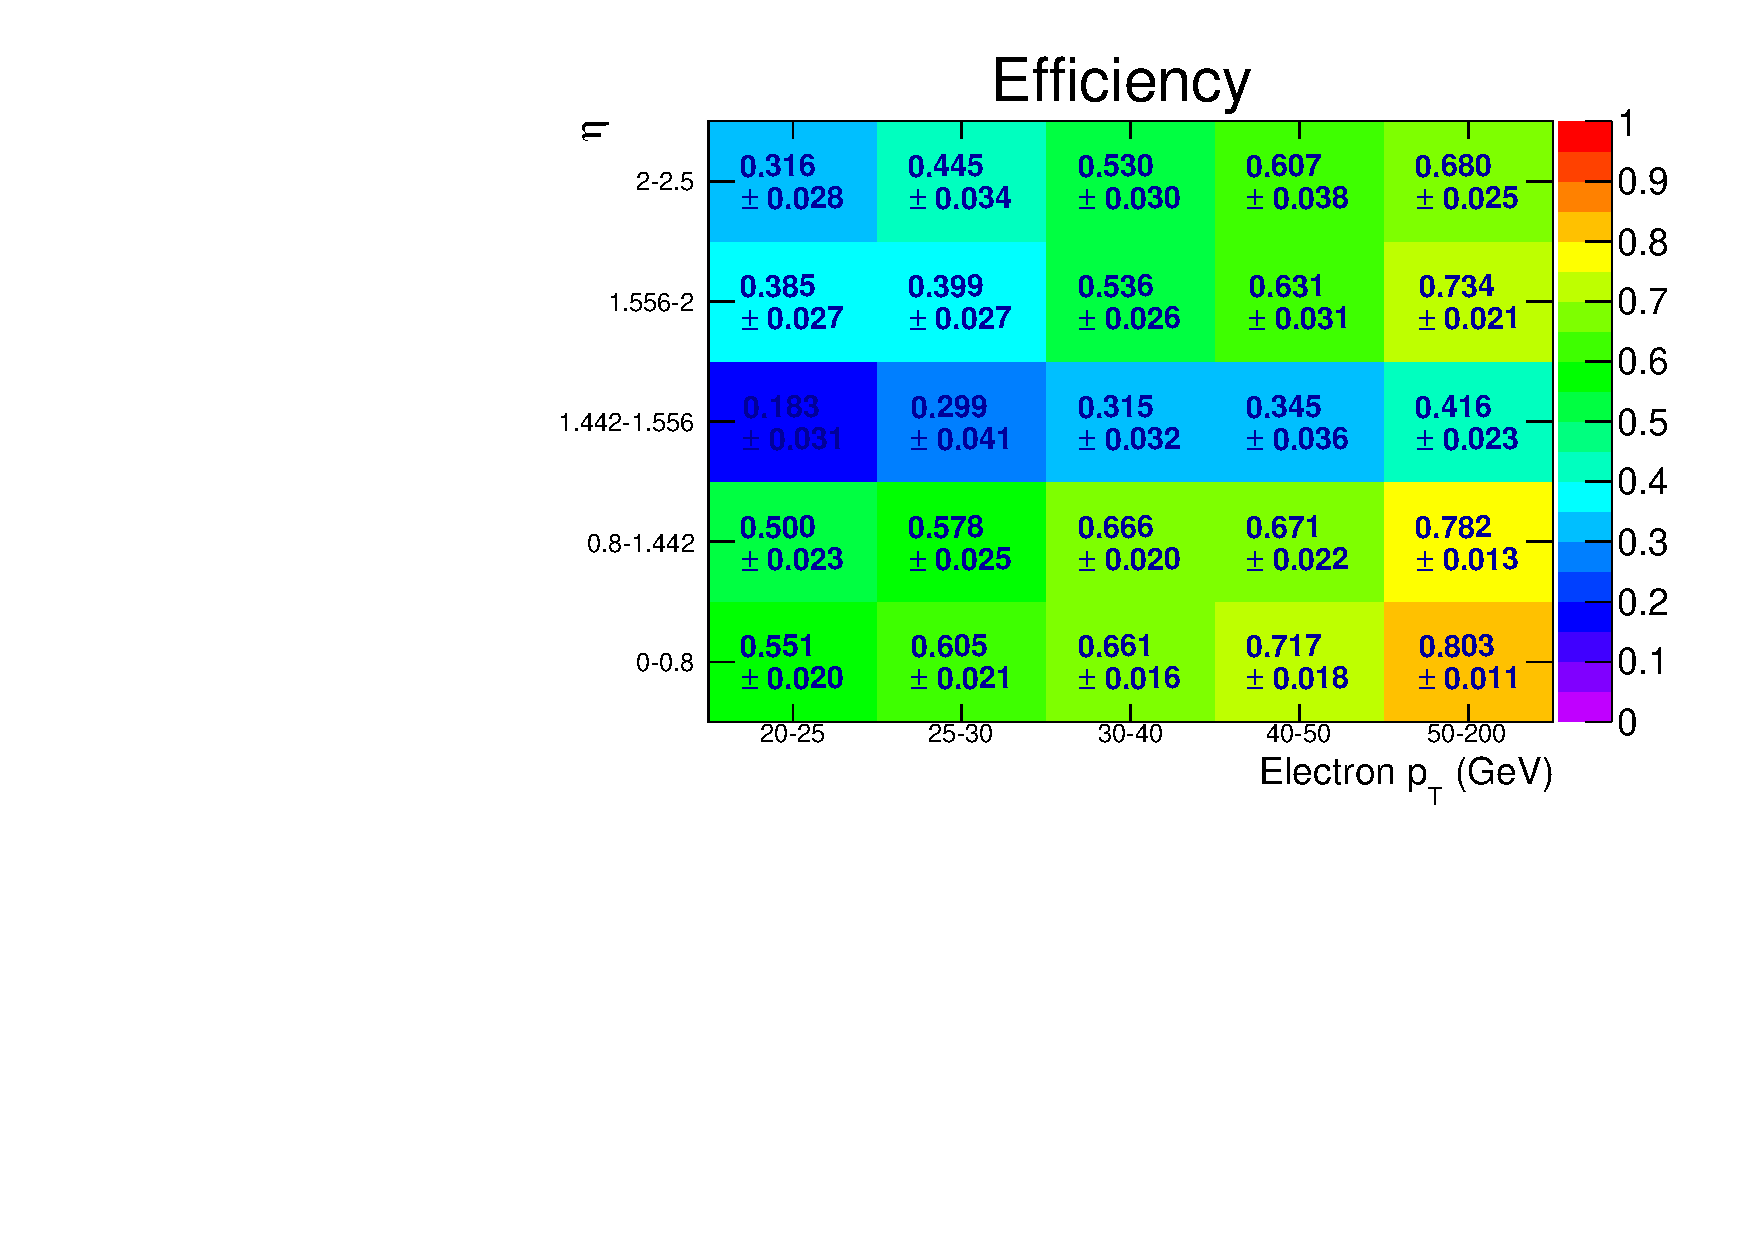
\includegraphics[angle=0,width=0.80\columnwidth]{fig/electron_eff.pdf}
\caption{The efficiency to select an analysis-level electron as a function of $\pT$ and $\eta$.}
\label{fig:electron_eff}
\end{figure}

\end{subsection}

\begin{subsection}{Muons}

The muon candidates are required to have $\pT > 20~\GeV$, $|\eta| < 2.4$, and to satisfy identification criteria~\cite{muon_id} in order to select a high purity muon sample.
This criteria is shown in Table~\ref{tab:muon_id}, where $d_0$ and $d_z$ are the transverse and logitudinal impact parameters of the associated muon track, respectively.
Analogously to electron candidates, muon candidates are required to satisfy $I^{\mrm{rel}} < 0.2$, where the looser threshold is to account for purity differences between electrons and muons.

\begin{table}[tb!]
\centering
\begin{tabular}{l|c}
\hline \hline
Criteria                                       &  Requirement \\
\hline
Is PF muon                                     &  True        \\
Fraction of valid tracker hits                 &  $> 0.8$     \\
\hline
\multicolumn{2}{c}{\texttt{AND}}                              \\      
$|d_0|$~[mm]                                   &  $< 2$       \\
$|d_z|$~[mm]                                   &  $< 5$       \\
Is global muon                                 &  True        \\
Normalized global-track $\chi^2$               &  $< 3$       \\
$\chi^2$ of tracker-standalone position match  &  $< 12$      \\
Track-kink $\chi^2$                            &  $< 20$      \\
Segment compatibility                          &  $> 0.303$   \\
\multicolumn{2}{c}{\texttt{OR}}                               \\
Segment compatibility                          &  $> 0.451$   \\
\hline\hline
\end{tabular}
\caption{Identification criteria that a PF muon must pass in order to be considered an analysis-level muon.}
\label{tab:muon_id}
\end{table}

The efficiency for reconstructing muons, shown in Figure~\ref{fig:muon_eff} is about 70\% at $\pT$ of $20~\GeV$, increasing to 80\% at $50~\GeV$, and reaching a plateau of 95\% for $\pT > 200~\GeV$~\cite{Chatrchyan:2012xi}.

\begin{figure}[tbp!]
\centering
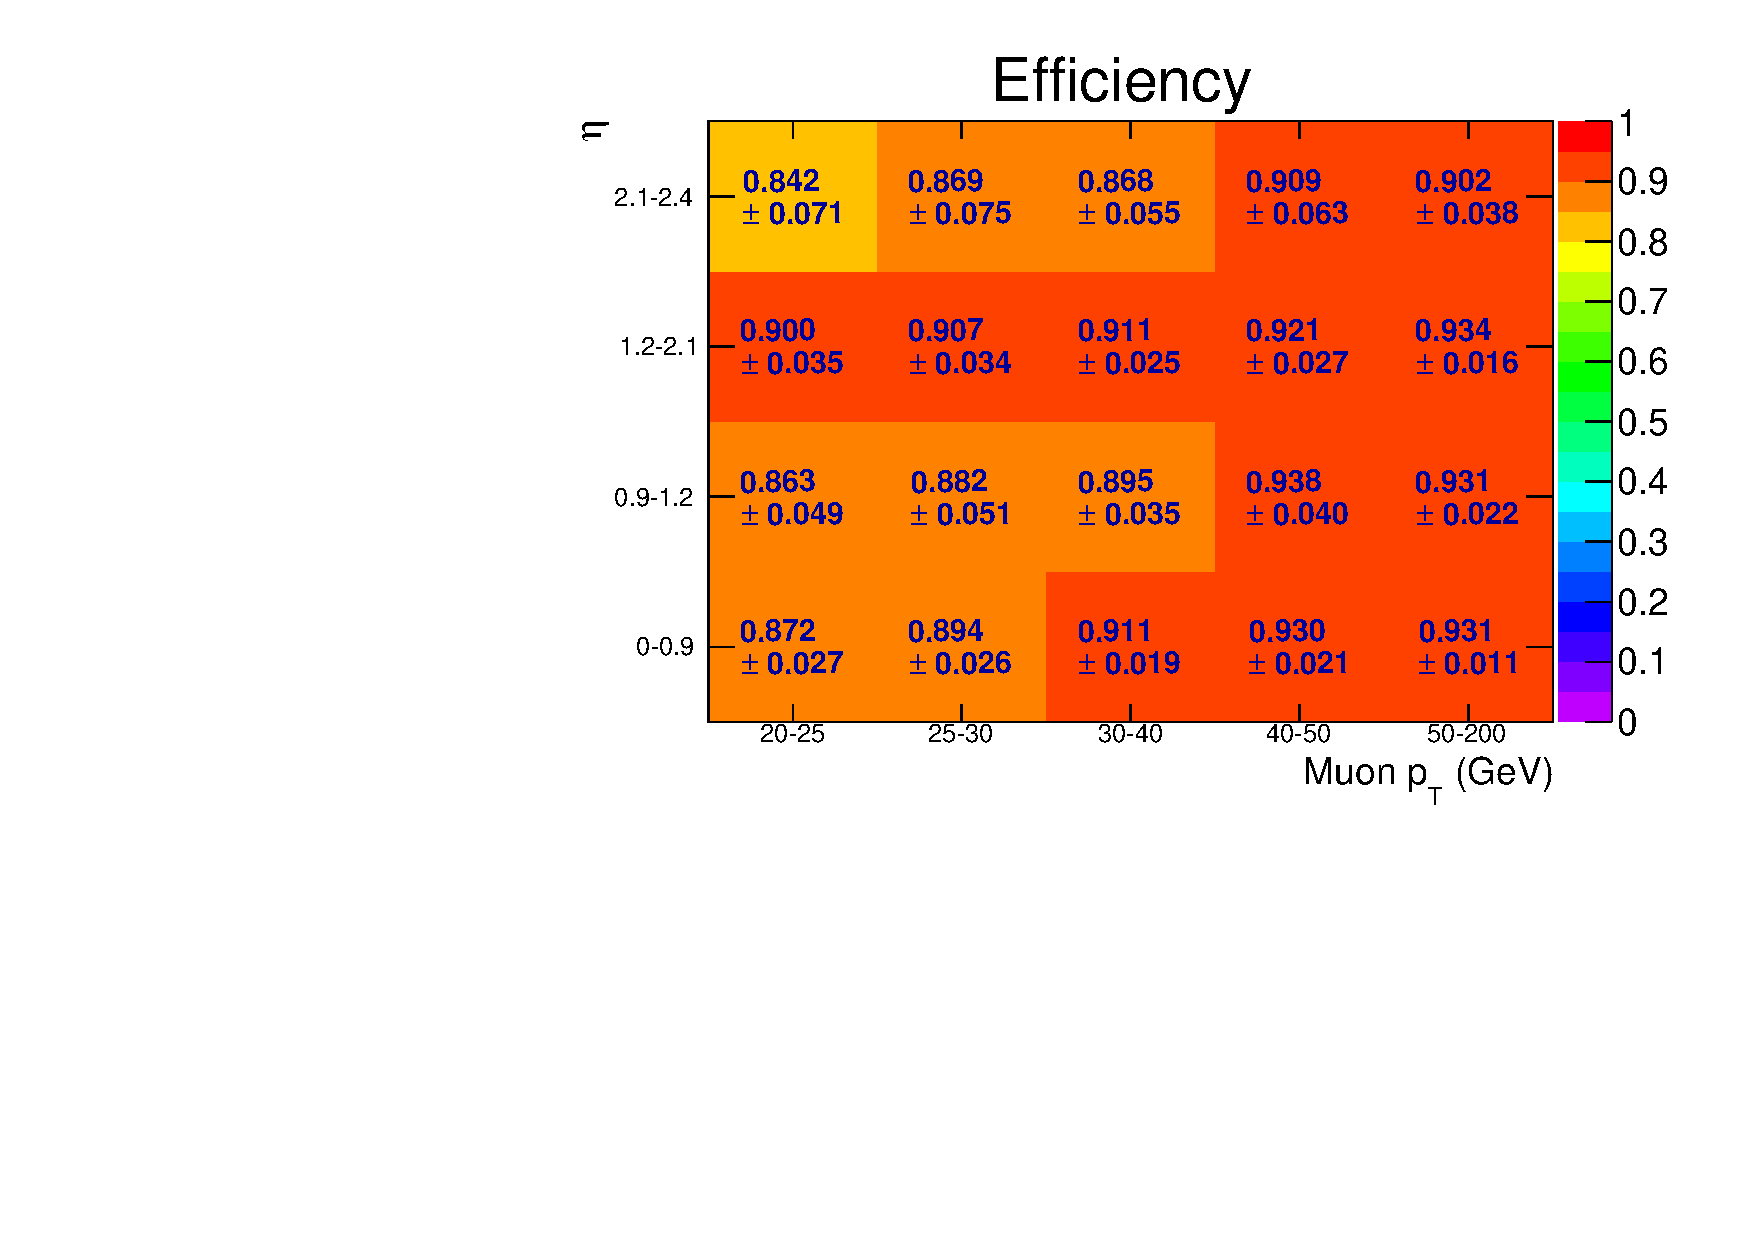
\includegraphics[angle=0,width=0.80\columnwidth]{fig/muon_eff.pdf}
\caption{The efficiency to select an analysis-level muon as a function of $\pT$ and $\eta$.}
\label{fig:muon_eff}
\end{figure}

\end{subsection}

\end{section}

\begin{section}{Jets}

When a quark or gluon is produced at the LHC, they quickly hadronize due to color confinement and produce a collimated ``spray'' of particles, called a jet, which is the direct detector observable.
The parameter of interest, however, is the momentum of the inital parton before hadronization.
Thus, clustering the constituent jet particles in a way that accurately reconstructs the inital parton momentum is essential.
Events, however, often contain multiple jets with each jet typically composed of some $\sim$$10$-$100$ particles that are incident on many detector channels across a large area.
This makes the problem of jet clustering non-trivial and an important aspect of object reconstruction.

\begin{subsection}{Clustering}

Jets are not physically-defined objects, and instead it is the clustering rules that define what a jet is.
The common class of clustering algorithms used are sequential recombination algorithms, which work by defining a distance measure between pairs of particles, typicaly based on energy and spatial-location, and then combining the closest pair of particles.
This process proceeds sequentially and ends when some threshold condition is met.

In particular, the distance measures, $d_{ij}$, which is the distance between two entities (particles or psuedojets), and $d_{iB}$, which is the distance between an entity and the beam, are often defined to be

\begin{equation}
d_{ij} = \mrm{min}(p_{\mrm{T}i}^{2p},p_{\mrm{T}j}^{2p})\frac{\Delta R_{ij}^{2}}{R^2},
\label{clustering_dij}
\end{equation}

\begin{equation}
d_{iB} = p_{\mrm{T}i}^{2p},
\label{clustering_diB}
\end{equation}

where $\Delta R_{ij}^{2} = \Delta \eta_{ij}^{2} + \Delta \phi_{ij}^2$, $R$ is the jet radius parameter that sets the scale of the jet's size, and $p$ is a parameter of the algorithm.
The clustering procedure then proceeds by finding the smallest of the distances, and if it is a $d_{ij}$, the two entities $i$ and $j$ are merged, while if it is a $d_{iB}$, entity $i$ is called a jet and is removed from the clustering list.

The parameter $p$ determines the clustering order of the algorithm and thus different choices for the value of $p$ lead to different clustering algorithms.
For $p = 1$, the clustering follows the \kT algorithm~\cite{Ellis:1993tq}, which prioritizes clustering softer particles first.
Setting $p = 0$, reproduces the Cambridge-Aachen algorithm~\cite{Dokshitzer:1997in}, which uses energy-independent clustering, relying only on the spatial distances between particles.
Lastly, choosing $p = -1$, gives the anti-\kT algorithm~\cite{Cacciari:2008gp}, which favors using the harder particles as the jet seeds and then clustering around them.
A more detailed discussion of jets, including a comparison of these and other clustering algorithms can be found in Reference~\cite{Salam:2009jx}.

\end{subsection}

\begin{subsection}{Selection}

The jets used in this dissertation are constructed by clustering PF candidates with the anti-\kT algorithm and $R = 0.4$, using the \textsc{FastJet} package~\cite{Cacciari:2011ma}.
To reduce the effect of pileup on the jet clustering and energy measurements, a process called ``Charged Hadron Subtraction'' is applied, where PF charged hadrons that do not originate from the PV are not included in the jet clustering.
In addtion, to remove the neutral energy component of pileup, the contribution from PF neutral hadrons produced by pileup is estimated based on the area of a jet and the energy density of the event and is subtracted from the jet~\cite{Cacciari:2007fd}.
Additionally, to prevent double-counting, any jets which contain a PF candidate identified as an analysis-level electron or muon are removed from the jet collection. 

Finally, to be considered an analysis-level jet, the jets must have $\pT > 30~\GeV$, $|\eta| < 2.4$, and must pass a set of loose identification requirements~\cite{jet_id,1748-0221-6-11-P11002} to surpress, for example, calorimeter noise.
These requirements are shown in Table~\ref{tab:jet_id}.
The resulting jets are considered to be ``\smallR'' jets  and the variable \Njets represents the number of these jets in an event.
Additionally, a proxy for the hadronic energy scale of an event, \HT, can be defined as
\begin{align}
\HT = \sum_{i = 1}^{\Njets} p_{T,i}^{jet}
\end{align}

\begin{table}[tb!]
\centering
\begin{tabular}{l|c}
\hline \hline
Criteria                          &  Requirement \\
\hline
Number of constituents            &  $> 1$       \\
Charged multiplicity              &  $> 0$       \\
Neutral electromagnetic fraction  &  $< 0.99$    \\
Neutral hadron fraction           &  $< 0.99$    \\
Charged electromagnetic fraction  &  $< 0.99$    \\
Chaged hadron fraction            &  $> 0$       \\
\hline\hline
\end{tabular}
\caption{Identification criteria that a jet candidate must pass in order to be considered an analysis-level jet.}
\label{tab:jet_id}
\end{table}

\end{subsection}

\begin{subsection}{b-tagging}

Jets that are formed through b-quark hadronization have many unique properties that allow them to be differentiated from jets formed through other quarks or gluons.
This abiilty to ``b-tag'' jets is a very useful tool for determining what physics processes occured in an event, as b~quarks are associated with specific physics process, such as top quark decays.
Similarly, many SUSY scenarios, where naturalness considerations motivate light third-generation squarks, result in either the direct or indirect production of b~quarks through the decay of SUSY particles.
Thus, b-tagging jets is not only often a crucial component to reducing backgrounds from processes where no b~quarks are expected, but also a powerful selector for potential signal events. 

This analysis uses the Combined Secondary Vertex v2 (CSVv2) algorithm~\cite{Chatrchyan:2012jua,Sirunyan:2017ezt}, which utilizes the long lifetimes, large masses, high-momentum daughter particles, and frequent semi-leptonic decays typical of b~hadrons to b-tag jets.
As the b~quark can only decay to an up or charm quark through highly Cabibbo surpressed weak interactions, b~hadrons tend to have long lifetimes, typically on the order of 150~\ps.
Because of this, b~mesons can travel a few mm to a cm from the PV before decaying and producing displaced tracks from which a secondary vertex can be reconstructed.
In addition, due to the relatively large b-quark mass, b~mesons tend to be heavy, which leads to both large secondary vertex masses and daughter particles with a hard momentum spectrum.
Lastly, the weak decay of the b~quark results in an associated electron or muon in about 20\% of decays.
The presence of these soft, nonisolated leptons provides an additional marker for the presence of a b-quark.

The CSVv2 algorithm exploits variables based on this information about secondary vertices, their associated displaced tracks, and the presence of soft leptons to accurately tag b-quark jets.
A selection of the variables used that have high discrimination are listed below:

\begin{itemize}
\item The significance of the flight distance in the transverse plane.
\item The number of SV
\item The SV mass
\item The number of tracks associated with the SV
\item The ratio of the transverse momentum of the SV tracks and the transverse momentum of the jet
\item The 3D impact parameter of soft leptons associated with the jet
\end{itemize}

These variables are then fed into a multilayer perceptron with one hidden layer then outputs a score between 0 and 1, indicating the likelihood the jet is a b-quark jet.
The distribution of CSVv2 disciminator values for different flavor jets is shown in Figure~\ref{fig:csv_discriminator}.

\begin{figure}[tbp!]
\centering
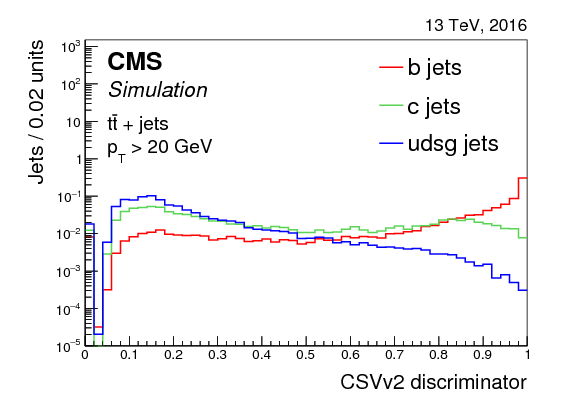
\includegraphics[angle=0,width=0.80\columnwidth]{fig/csv_discriminator.png}
\caption{The distribution of the CSVv2 discriminator values for jets of different flavors.
Jets are selected from \ttbar events and required to have $\pT > 20~\GeV$~\cite{Sirunyan:2017ezt}.}
\label{fig:csv_discriminator}
\end{figure}

A threshold score for b-tagging a jet is chosen such that the mis-tag rate for light-flavor jets is 1\%.
This corresponds to a mis-tag rate for c-quark jets of 13--15\% (11--13\%) in the barrel (endcap) and a tagging efficiency for b~jets of 60--67\% (51--57\%) in the barrel (endcap) for jets with \pT between $30$-$50~\GeV$.
The tagging efficiency increases with \pT before decreasing to $\approx 50\%$ for jets above $150~\GeV$.
The b-tagging efficiency as a function of jet \pT is shown in Figure~\ref{fig:btag_eff}.

The number of b-tagged jets in an event is denoted as \Nb.

\begin{figure}[tbp!]
\centering
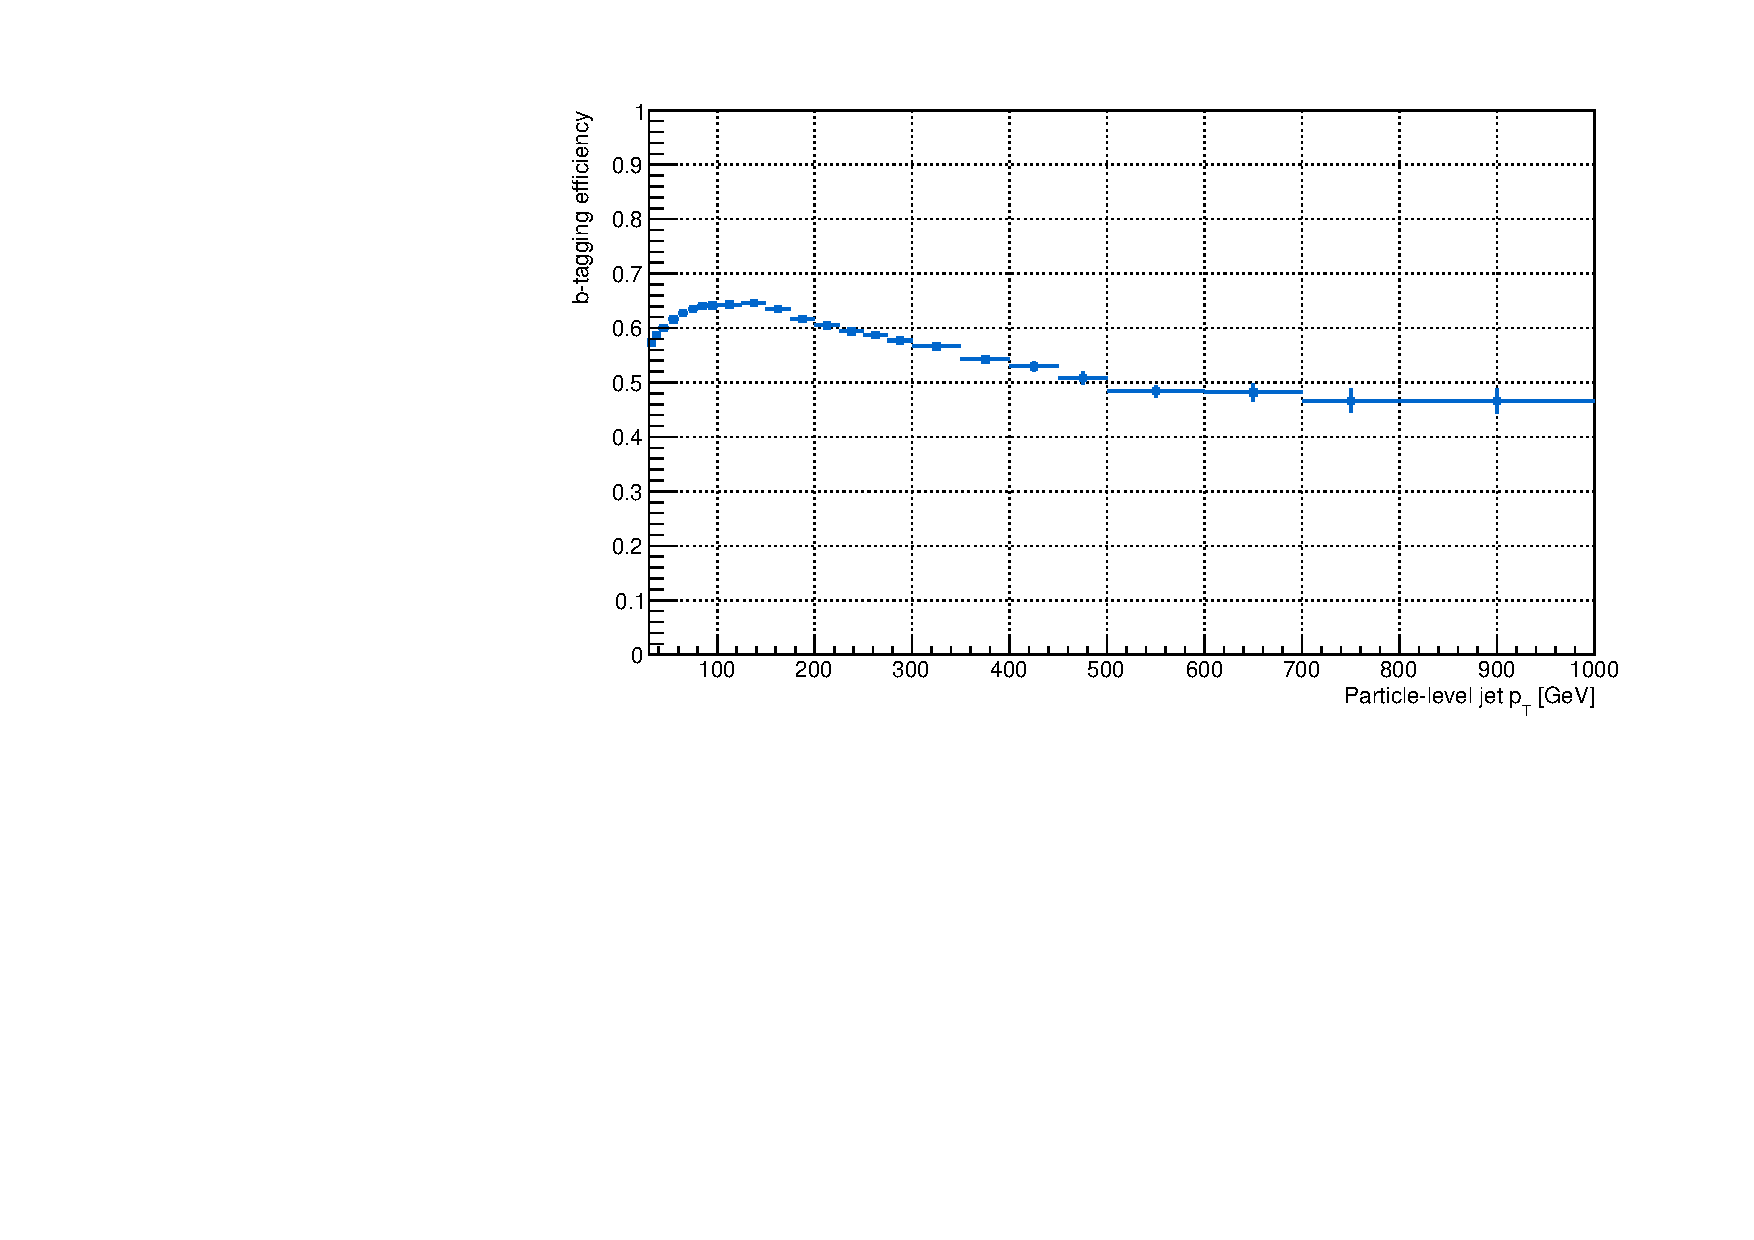
\includegraphics[angle=0,width=0.80\columnwidth]{fig/btag_eff.pdf}
\caption{The efficiency of the CSVv2 algorithm as a function of jet \pT at the working point used in this analysis.}
\label{fig:btag_eff}
\end{figure}

% SHOW VARIABLE PLOTS: https://inspirehep.net/record/1644362/plots

\end{subsection}

\end{section}

\begin{section}{Large-radius Jets}

While the distance parameter of \smallR jets is optimized for clustering the hadronization products of a single parton, it is often useful to exploit information of physical processes on scale larger than a single jet, such as top quark or W boson decays.
One way to capture this information is to cluster jets with a large distance parameter, which encodes the momentum, angular, and multiplicity information of the partons contained in this larger jet.

In particular, this analysis constructs these ``\largeR'' jets by clustering ``\smallR'' jets with a distance parameter of $R = 1.2$.
Due to the relatively small number of \smallR jets in an event ($\lesssim 10$), the construction of these \largeR jets is insensitive to the clustering algorithm, and the anti-\kT algorithm is chosen.
While these \largeR jets could be constructed by performing the clustering at the PF candidate level, no significant improvement in performance was noted.
Thus, clustering \smallR jets were chosen for the following practical considerations.
First, the \textsc{FastJet} implementation of the anti-\kT algorithm has complexity $\mathcal{O}(n\log n)$~\cite{Cacciari:2005hq}, which results in a speed-up of on the order of 100x when clustering \smallR jets ($\lesssim 10$ objects) compared to PF candidates ($\sim$1000 objects).
Secondly, \largeR jets clustered from PF candidates would require the computation of new energy-measurement and pileup-removal calibrations for jets of this specific radius.
Small-$R$ jets, however, already incorporate standardized calibrations and by clustering these calibrated \smallR jets, the \largeR jets correspondingly incorporate corrections without the need of any additional development.

In addition to \smallR jets, the jets associated with selected leptons are included in the formation of \largeR jets in order to capture as much of an event's kinematic information as possible.
For example, this helps reduce the difference between \largeR jets formed by clustering hadronic and (semi-)leptonic decays, as by including the lepton, the only information difference between the two scenarios is due to the undetected neutrino(s).

This technique of clustering \smallR jets into \largeR jets has been used previously by both the ATLAS and CMS collaborations, e.g. References~\cite{Aaboud:2017aeu,Khachatryan:2016uwr}.

\begin{subsection}{\MJ}
\label{subsec:MJ}

A measure of the mass-scale of an event, \MJ, can be constructed by summing the masses of large-radius jets, defined as
\begin{align}
\MJ = \sum_{J_{i}\, \in\, {\text{large-}R\text{ jets}}} m(J_i)
\end{align}
where $m(J)$ is the mass of a single \largeR jet.

The quantitity \MJ has significant discriminating power between SM background processes and signal processes, as SM events tend to have significantly lower mass-scales than signal events that involve high mass particles.
For example, \MJ in events with only a produced \ttbar pair is limited to be $\lesssim 2m_{top} \approx 350~\GeV$.
This is because the top quarks decay back-to-back and if each top quark's decay products are captured in a single \largeR jet, two \largeR jets are clustered each with $m(J) = m_{top}$, resulting in $\MJ = 2m_{top}$.
In the case, where a top quark is not fully contained in a \largeR jet, the mass of that \largeR jet, and correspondingly \MJ, is even smaller.
For signal events, however, the mass-scale is roughly set by the gluino mass, which is on the order of $1~\TeV$.

The \MJ distribution in \ttbar and signal events with $\mglu = 1000~\GeV$ and $1600~\GeV$, selected with a $\Njets \geq 8$ requirement to ensure both processes have similar \Njets distributions, is shown in Figure~\ref{fig:mj_distributions}. 
From the figure, it can be seen that the \MJ distribution gets increasingly harder with higher gluino mass.
Also of note is that the \MJ distribution in \ttbar events extends past $2m_{top}$.
This is because, in the presence of significant ISR, the ISR jets can either overlap with the \ttbar daughter jets or boost the \ttbar system such that the system is collimated, both which result in high-mass \largeR jets and, correspondingly, high-\MJ.
Processes of this nature are responsible for generating high \MJ background events.

The quantity \MJ was proposed in phenomenological studies~\cite{Hook:2012fd,Cohen:2012yc,Hedri:2013pvl} and was first used for RPC SUSY searches by the ATLAS Collaboration in all-hadronic final states~\cite{Aad:2015lea,Aad:2013wta} and by the CMS Collaboration in single-lepton events~\cite{Khachatryan:2016uwr,Sirunyan:2017fsj}.
Additionally, the basic properties and performance of the \MJ variable were commissioned using early $\sqrt{s} = 13~\TeV$ data~\cite{CMS-DP-2015-035}.

\begin{figure}[tbp!]
\centering
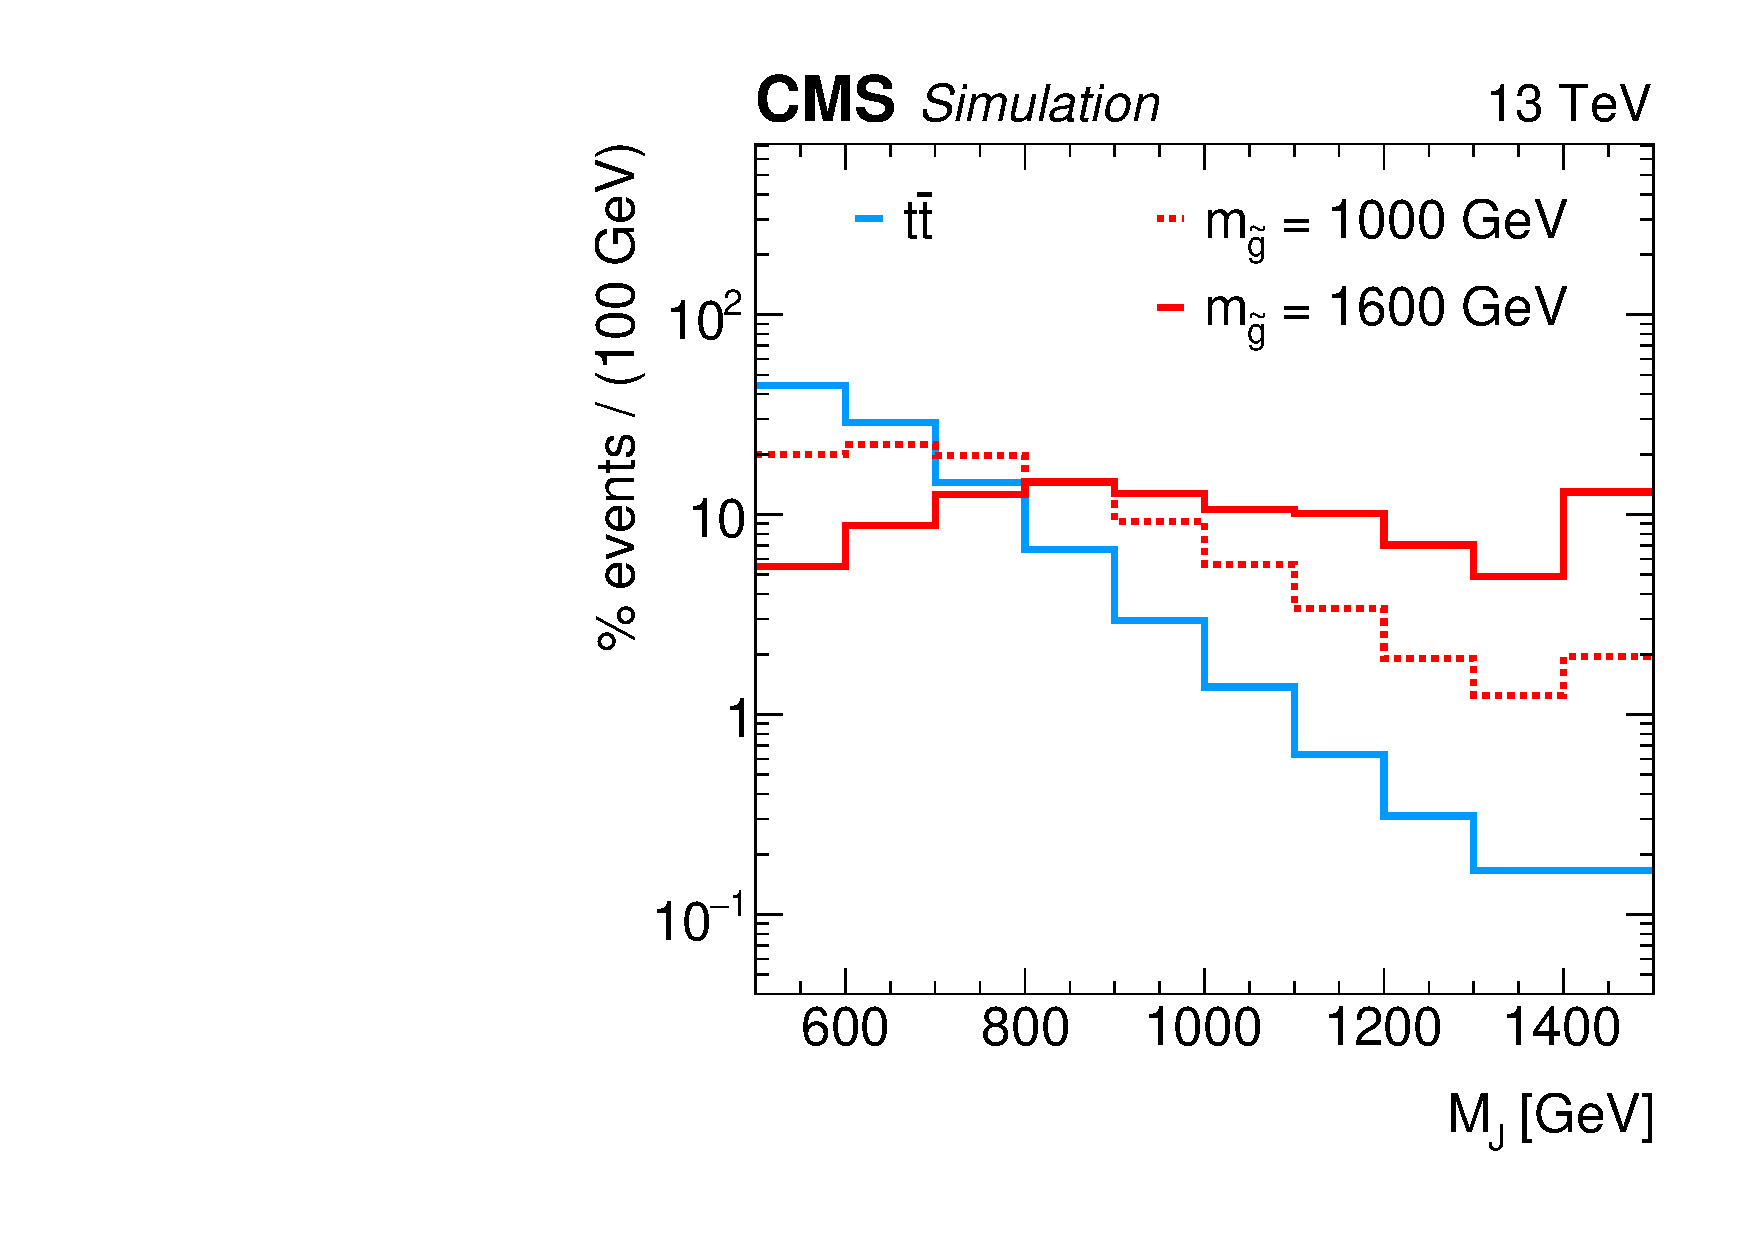
\includegraphics[angle=0,width=0.80\columnwidth]{fig/mj_distributions.pdf}
\caption{Distributions of \MJ, normalized to the same area, for \ttbar events and signal events with $\mglu = 1000~\GeV$ and $1600~\GeV$ in a selection of \baseNleps, \baseHT, $\Njets \geq 8$, \baseMJ, and \baseNb.}
\label{fig:mj_distributions}
\end{figure}

\end{subsection}

\end{section}
